\documentclass[a4paper, 11pt]{article}

\usepackage[absolute]{textpos} % absolute positioned text blocks
\setlength{\TPHorizModule}{1mm}
\setlength{\TPVertModule}{1mm}
\usepackage[english]{babel}
\usepackage{csquotes}

% Images
\usepackage{graphicx} % used for images
\graphicspath{ {./../img/} }
\usepackage[labelfont=bf]{caption}

% Formatting
\usepackage{geometry} % better margins for document
\usepackage{titlesec} % better control over title spacing 
\usepackage{tabularx} % better tables
\usepackage[hidelinks]{hyperref} % hrefs
\usepackage{totcount}
\usepackage{float} % image placement

% Code listings
\usepackage{listings}
\usepackage{xcolor}
\definecolor{codered}{rgb}{0.95,0.42,0.458}
\definecolor{codegrey}{rgb}{0.7,0.7,0.7}
\definecolor{codepink}{rgb}{0.737,0.47,0.823}
\definecolor{codeblue}{rgb}{0.227,0.572,0.937}
\definecolor{codegreen}{rgb}{0.341,0.664,0.2}
\definecolor{codestring}{rgb}{0.58,0,0.82}
\definecolor{backcolor}{rgb}{0.95,0.95,0.95}
\lstdefinelanguage{HLSL}{
	morekeywords=[1]{
        position,sphere,direction,stepSize,dirMultiplier,distanceScene,distanceOrigin,p,
	},
	morekeywords=[2]{
		distance,normalize,
		sphereHit,raymarch,sphereDistance,sdf,estimateNormal,
	},
	morekeywords=[3]{
		STEP_SIZE,MAX_STEPS,MINIMUM_STEP_SIZE,SURFACE_DISTANCE,MAX_DISTANCE,E,
    },
    keywordstyle=[1]\color{codeblue},
    keywordstyle=[2]\color{codered},
    keywordstyle=[3]\color{codepink},
	commentstyle=\color{codegrey},
	morestring=[b]", % defines that strings are enclosed in double quotes
	morestring=[b]', % defines that strings are enclosed in single quotes
    backgroundcolor=\color{backcolor},
    stringstyle=\color{codered},
    numberstyle=\tiny,
    basicstyle=\ttfamily\footnotesize,
    breakatwhitespace=false,
    breaklines=true,
    captionpos=b,
    keepspaces=true,
    numbers=left,
    numbersep=5pt,
    showspaces=false,
    showstringspaces=false,
    showtabs=false,
	tabsize=2,
    sensitive=false, % keywords are not case-sensitive
    morecomment=[l]{//}, % l is for line comment
    morecomment=[s]{/*}{*/}, % s is for start and end delimiter
    belowskip=2.5em,
    aboveskip=1em,
}

% Gantt charts
\usepackage{pgfgantt}

% drawings
\usepackage{tikz}
\usetikzlibrary{arrows.meta}

\geometry{
	a4paper,
	left=28mm,
	right=28mm,
    top=30mm,
    bottom=30mm
}

% Colors 
\RequirePackage{color}
\definecolor{bfhgrey}{rgb}{0.41,0.49,0.57}

% Glossary
\usepackage[toc]{glossaries}
\newacronym{hlsl}{HLSL}{ High Level Shading Language }
\newacronym{gpu}{GPU}{ Graphics Processing Unit }
\newglossaryentry{latex}{name=LaTeX, description={ A high-quality document preparation system designed for the production of technical and scientific documentation }}
\newglossaryentry{noisegeneration}{name=Noise generation, text={noise generation}, description={ Noise generation is used to generate textures of one or more dimension with seemingly random smooth transitions from black to white (zero to one) }}
\newglossaryentry{volumetricrendering}{name=Volumetric rendering, text={volumetric rendering}, description={ This describes a technique which takes a 3D volume of data and projects it to 2D. It is mostly used for transparent effects stored as a 3D image }}
\newglossaryentry{raymarching}{name=Ray marching, text={ray marching}, description={ Ray marching is a type of method to approximate the surface distance of a volumetric object, where a ray is cast into the volume and stepped forward until the surface is reached }}
\newglossaryentry{lightmarching}{name=Lightmarching, text={lightmarching}, description={ The same concept as \gls{raymarching}, but instead of being cast into the volume, it is cast towards the primary light source with a constant step }}
\newglossaryentry{convection}{name=Convection, text={convection}, description={ Convection describes the transfer of heat from movement of liquid or gas }}
\newglossaryentry{billboard}{name=Billboard, text={billboard}, description={ A 2D image always facing towards the main camera }}
\newglossaryentry{worldspace}{name=World space, text={world space}, description={ Coordinates defined with respect to a global Cartesian coordinate system }}
\newglossaryentry{polymesh}{name=Polymesh, text={polymesh}, description={ A polymesh is a 3D model composed of polygons or triangles }}
\newglossaryentry{lowpoly}{name=Low poly, text={low poly}, description={ A 3D polymesh with a relatively low count of polygons }}
\newglossaryentry{voxel}{name=Voxel, text={voxel}, description= { Short for \textit{volume element}, a voxel is a value (either a number or a vector) on a scalar or vector field }}
\newglossaryentry{scalarfield}{name=Scalar field, text={scalar field}, description={ A scalar field describes a typically three-dimensional grid of elements called \textit{voxels}, each containing a scalar value }}
\newglossaryentry{vectorfield}{name=Vector field, text={vector field}, description={ It is the same as a scalar field, except the voxels are vector values }}
\newglossaryentry{spheretracing}{name=Sphere tracing, text={sphere tracing}, description={ Sphere tracing describes an optimized algorithm of ray marching by using signed distance functions to approximate the surface distance of the volume }}
\newglossaryentry{sdf}{name=Signed distance function, text={signed distance function}, description={ A signed distance function, short SDF, returns a positive distance if the origin is outside the volume and a negative distance if it is inside the volume }}
\newglossaryentry{surfacenormal}{name=Surface normal, text={surface normal}, description={ A \textit{surface normal} or \textit{normal} is a vector which is perpendicular to a given geometry, like a triangle or polygon }}
\newglossaryentry{gradient}{name=Gradient, text={gradient}, description={ The \textit{gradient} denotes the direction of the greatest change of a scalar function }}
\newglossaryentry{penumbra}{name=Penumbra, text={penumbra}, description={ The partially shaded outer region of diffuse shadows. Also described as soft edges }}
\newglossaryentry{shapeblending}{name=Shape blending, text={shape blending}, description={ In SDFs, shapes can be seemingly blended together by returning a interpolated value of those distances }}
\newglossaryentry{ambientocclusion}{name=Ambient occlusion, text={ambient occlusion}, description={ Also known as contact shadows, this method darkens points in the scene that are not or only slightly exposed to the light and its environment }}
\newglossaryentry{noise}{name=Noise, text={noise}, description={ A randomly generated pattern, referring to \gls{procedural} pattern generation }}
\newglossaryentry{translucent}{name=Translucent, text={translucent}, description={ An object or substance that is translucent allows light to be passed through it, meaning it is rendered transparently to some degree }} 
\newglossaryentry{parameters}{name=Parameters, text={parameters}, description={ Shader variables exposed to the Unity Editor }} 
\newglossaryentry{sss}{name=Subsurface scattering, text={subsurface scattering}, description={ SSS is a mechanism of light transport in which light enters a translucent object, is scattered around and exits the material at a different point, resulting in illuminated areas where the material is thin }} 
\newglossaryentry{sunlightforwarding}{name=Sunlight forward scattering, text={sunlight forward scattering}, description={ The process of sunlight shining through and illuminating the clouds which cover the sun }} 
\newglossaryentry{sunlighttransmittance}{name=Sunlight transmittance, text={sunlight transmittance}, description={ In this matter, the same as \gls{sunlightforwarding} }} 
\newglossaryentry{cnn}{name=Convolutional neural network, text={convolutional neural network}, description={ A neural network that is able to classify images }} 
\newglossaryentry{gan}{name=Generative adverserial network, text={generative adverserial network}, description={ A set of two neural networks, where one generates images and the other tries to tell wether those images are real or generated }} 
\newglossaryentry{aabb}{name=Axis-aligned bounding box, text={axis-aligned bounding box}, description={ A non-rotated bounding box enclosing an object completely }} 
\newglossaryentry{computeshader}{name=Compute shader, text={compute shader}, description={ A shader which runs on the GPU but outside of the default render pipeline }} 
\newglossaryentry{fbm}{name=Fractal Brownian motion, text={fractal Brownian motion}, description={ Different iterations of continuously more detailed noise layered on top of each other }} 
\newglossaryentry{fractalnoise}{name=Fractal noise, text={fractal noise}, description={ In this matter, the same as \gls{fbm} }} 
\newglossaryentry{procedural}{name=Procedural, text={procedural}, description={ Created solely with algorithms and independant of any prerequisites }}
\newglossaryentry{histogram}{name=Histogram, text={histogram}, description={ A graphical representation of data like brightness or color distribution of a given photograph }}
\newglossaryentry{csg}{name=Constructive solid geometry, text={constructive solid geometry}, description={ Short CSG, stands for combining primitive geometric objects with Boolean operators }}
\makenoidxglossaries

% Bibliography
\usepackage[backend=biber, style=ieee]{biblatex}
\addbibresource{partials/specification.bib}

% add another lavel of headings
\setcounter{secnumdepth}{4}
\setcounter{tocdepth}{3}
\titleformat{\paragraph}
{\normalfont\normalsize\bfseries}{\theparagraph}{1em}{}
\titlespacing*{\paragraph}
{0pt}{3.25ex plus 1ex minus .2ex}{1.5ex plus .2ex}

\begin{document}

\color{black}

\title{\doctitle}
\author{\docauthor}
\date{\versiondate}

\newcounter{requirements}
\newtotcounter{versionnumber}
\newcommand{\docsubtitle}{Project documentation}
\newcommand{\docauthor}{Matthias Thomann}
\newcommand{\doctitle}{Procedural cloud shader}
\newcommand{\fieldofstudies}{BSc in Computer Science}
\newcommand{\specialisation}{Computer perception and virtual reality}
\newcommand{\prof}{Prof. Urs K\"unzler}

\newcommand{\versiondate}{\today}
\newcommand{\sectionref}[1]{\autoref{#1}}
\newcommand{\emptyline}{\vspace{\baselineskip}\\\noindent}

\titlespacing*{\section} {0pt}{7.5ex plus 1ex minus .2ex}{2.3ex plus .2ex}
\titlespacing*{\subsection} {0pt}{4.25ex plus 1ex minus .2ex}{1.5ex plus .2ex}

\pagenumbering{roman}
\setcounter{page}{3}

%% include BFH logo and HuCE-ml logo

\begin{titlepage}

\setlength{\unitlength}{1mm}

\begin{textblock}{20}[0,0](22,12)
    
\includegraphics[scale=1.0]{../img/BFH_Logo_B.png}
\end{textblock}

\begin{flushleft}

\vspace*{21mm}

\fontsize{26pt}{40pt}\selectfont
\textbf{\doctitle}	\\
\vspace{2mm}

\fontsize{16pt}{24pt}\selectfont\vspace{0.3em}
\docsubtitle
\vspace{5mm}

\fontsize{10pt}{12pt}\selectfont
\textbf{Project 2} \\

\fontsize{10pt}{12pt}\selectfont
The goal of this project is to research and implement a procedural, volumetric cloud shader. The following document reveals the process of creating such a shader from both a technical and mathematical perspective, considering different algorithms for techniques like noise generation and raymarching.
\begin{textblock}{150}(28,225)
\fontsize{10pt}{17pt}
\begin{tabbing}
xxxxxxxxxxxxxxxxxxxxx\=xxxxxxxxxxxxxxxxxxxxxxxxxxxxxxxxxxxxxxxxxxxxxxx \kill
Field of Studies:	\> \fieldofstudies	\\
Specialization:	    \> \specialisation	\\
Author:		        \> \docauthor \\
Supervisor:         \> \prof \\
Date:			    \> \versiondate \\
\end{tabbing}

\end{textblock}

\begin{textblock}{150}(28,280)
\noindent 
\color{bfhgrey}\fontsize{9pt}{10pt}\selectfont
Berner Fachhochschule | Haute \'ecole sp\'ecialis\'ee bernoise | Bern University of Applied Sciences
\color{black}\selectfont
\end{textblock}

\end{flushleft}

\end{titlepage}

\clearpage


\tableofcontents
\clearpage

\pagenumbering{arabic}

\nocite{online:realtime-volumetric-cloudscapes}
\nocite{online:volumetric-cloudscapes}
\nocite{online:raymarching-sdf}
\nocite{online:volumetric-rendering}

\section{General}

\subsection{Purpose}
During this project, all gathered information and knowledge about the researched algorithms and techniques are written down in this document.

\subsection{Revision History}
\begin{tabularx}{\textwidth}{|c|c|c|X|}
    \hline
    \textbf{Version}         & \textbf{Date}     & \textbf{Name}     & \textbf{Comment}                  \\ \hline \addtocounter{versionnumber}{1}
    0.\arabic{versionnumber} & March 21, 2020    & Matthias Thomann  & Initial draft                     \\ \hline \addtocounter{versionnumber}{1}
    0.\arabic{versionnumber} & March 29, 2020    & Matthias Thomann  & Added first research results      \\ \hline
\end{tabularx}
\clearpage

\section{Natural Clouds}

\subsection{Formation}
Clouds, as seen in nature, consist of of a visible body of tiny water droplets and frozen crystals. 
In their natural occurence, clouds are mostly generated from a nearby source of moisture, usually in the form of water vapor. 
This composition of particles creates the pleasant look of a white-grayish "fluffy" mass, floating in the sky.
\\
Due to certain factors like altitude or water source, different types of cloudscapes can be formed. They vary in shape, \gls{convection}, density and more.
That makes different cloudscapes highly unique in terms of appearance.
\\
For now, those factors are regarded as nature's randomness. However, an approximation of randomness will be covered in \sectionref{section:noise-generation}.


\subsection{Types of Clouds}
\label{section:cloud-types}
Cloudscapes are classified in multiple groups, mainly differing in altitude, meaning the distance from the earth's surface to the cloud formation.
The following four cloud genera stand out due to their distinctiveness. A realistic simulation of a cloud system would consist of a combination of these types, which is why they are displayed here.
\begin{figure}[ht]
    \centering
        \begin{minipage}{0.47\linewidth}
            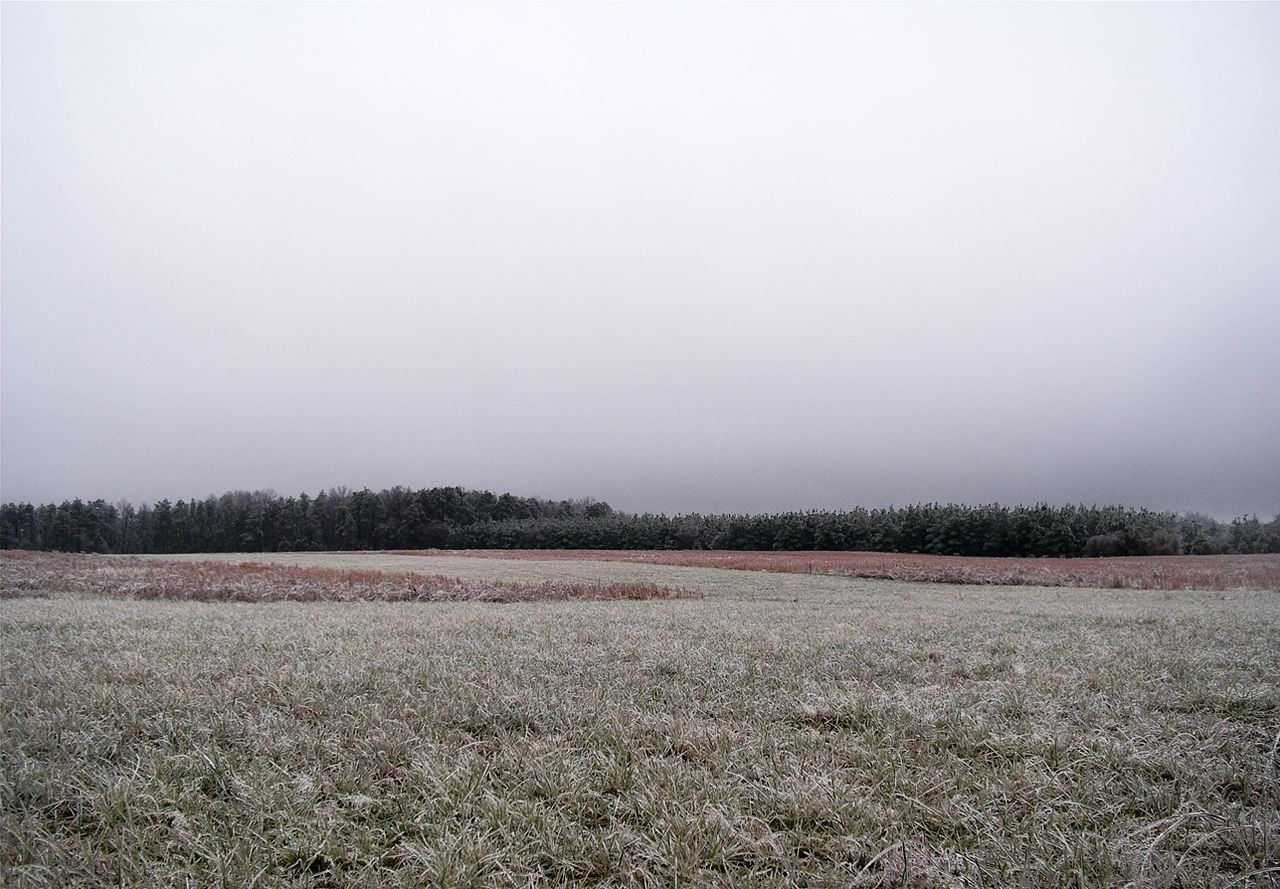
\includegraphics[width=\linewidth]{cloudforms-stratus}
            \captionof{figure}{Photographic reference of stratus clouds \protect\cite{img:cloudforms:stratus}.}
            \label{img:photo:cloudforms-stratus}        
        \end{minipage}        
    \hfill
        \begin{minipage}{0.47\linewidth}
            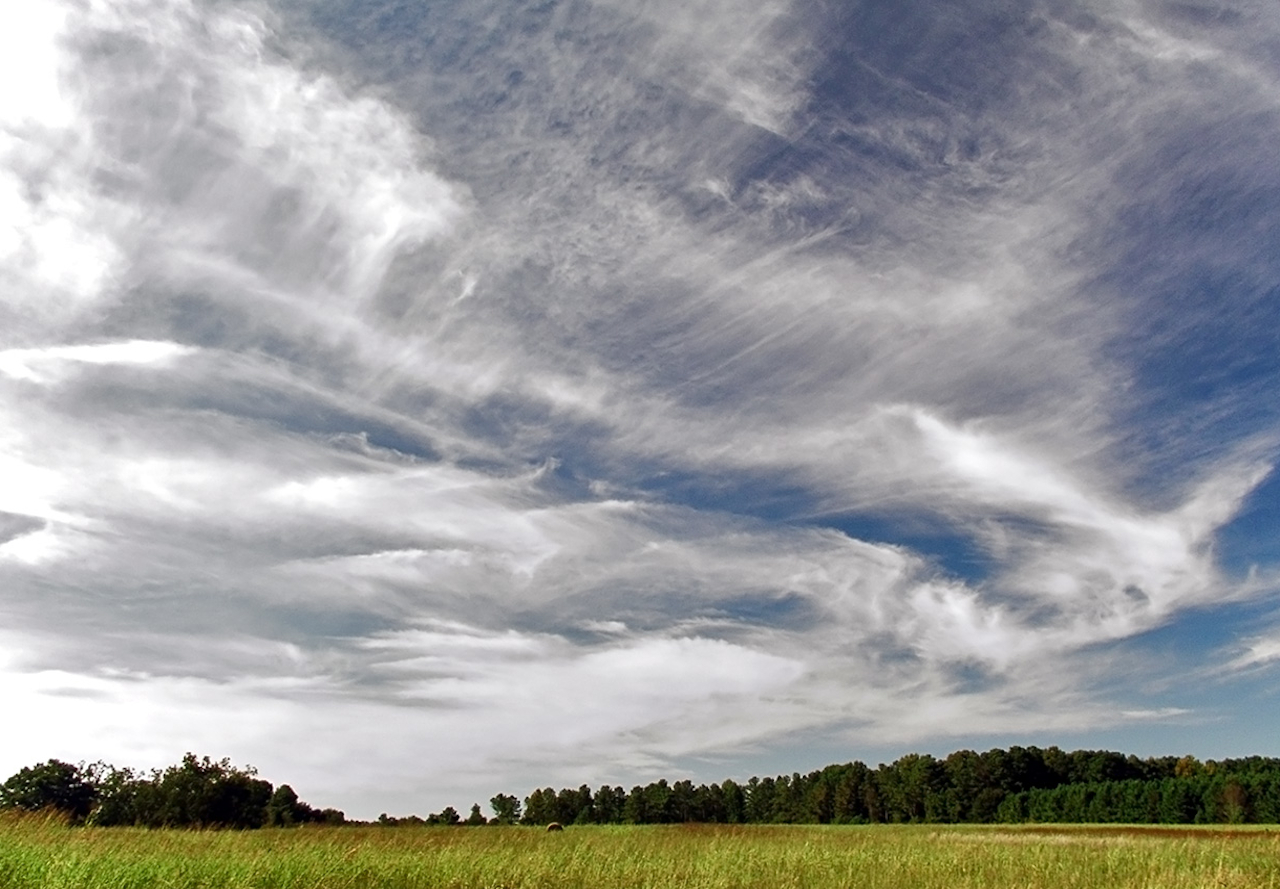
\includegraphics[width=\linewidth]{cloudforms-cirrus}
            \captionof{figure}{Photographic reference of cirrus clouds \protect\cite{img:cloudforms:cirrus}.}
            \label{img:photo:cloudforms-cirrus}        
        \end{minipage}
\end{figure}

\begin{figure}[ht]
    \centering
        \begin{minipage}{0.47\linewidth}
            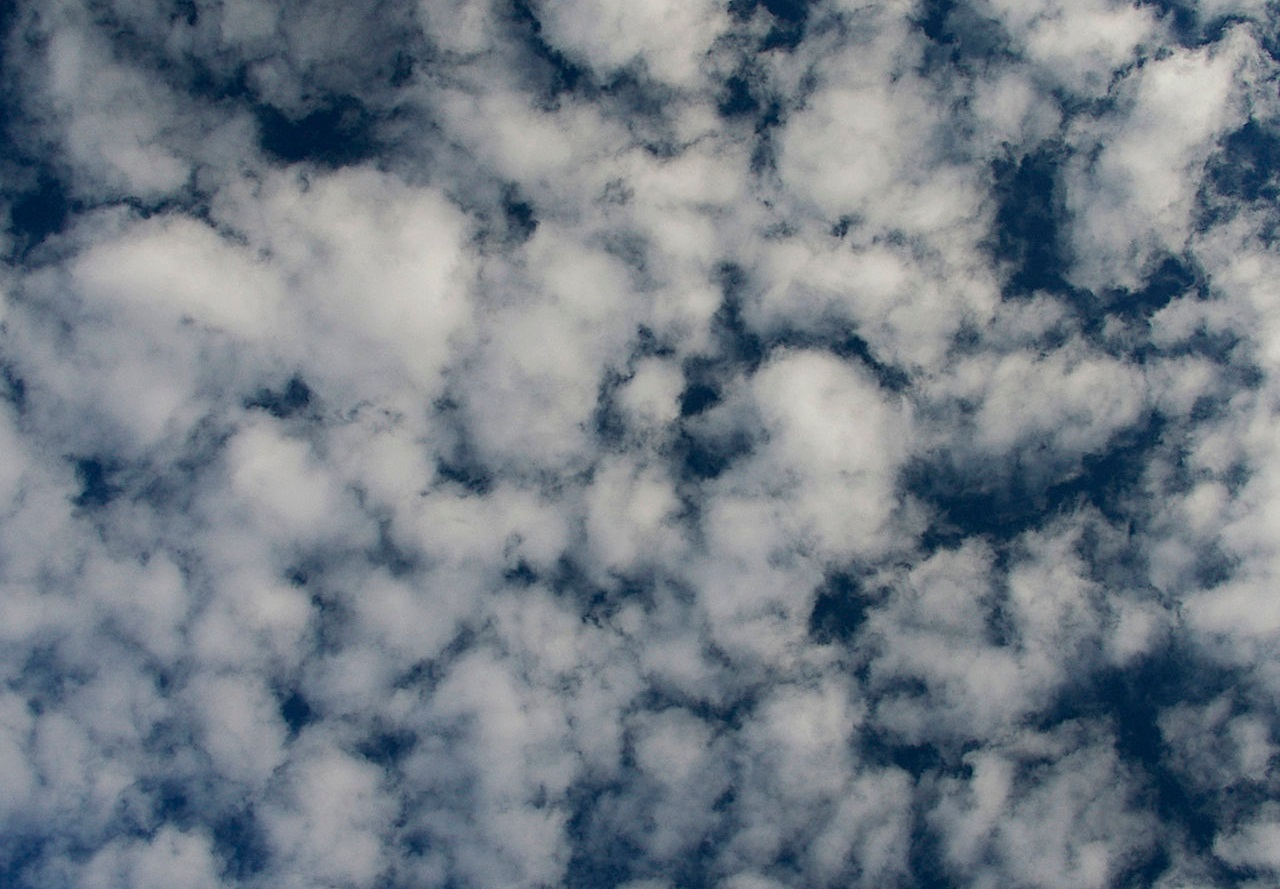
\includegraphics[width=\linewidth]{cloudforms-altocumulus}
            \captionof{figure}{Photographic reference of an altocumulus cloud formation \protect\cite{img:cloudforms:altocumulus}.}
            \label{img:photo:cloudforms-altocumulus}        
        \end{minipage}        
    \hfill
        \begin{minipage}{0.47\linewidth}
            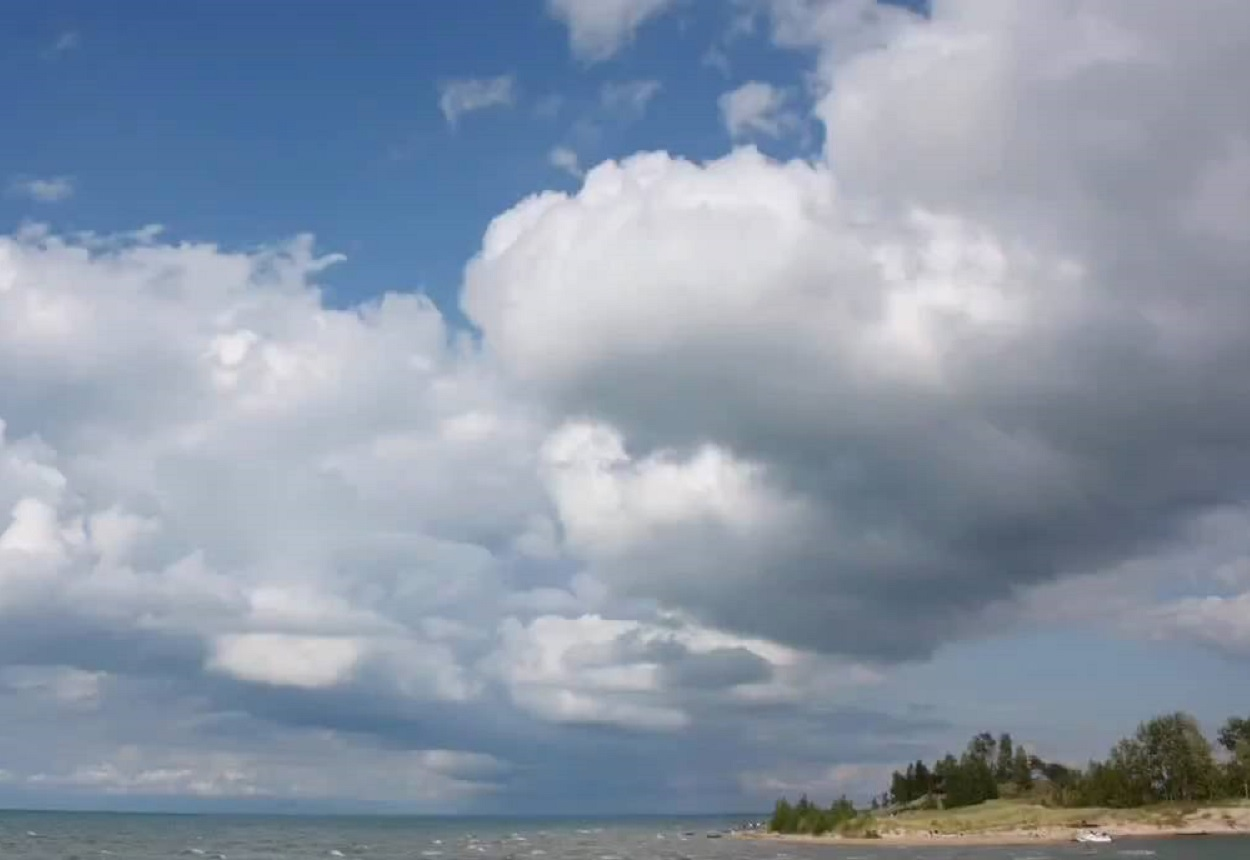
\includegraphics[width=\linewidth]{cloudforms-stratocumulus}
            \captionof{figure}{Photographic reference of stratocumulus cloudscape \protect\cite{img:cloudforms:stratocumulus}.}
            \label{img:photo:cloudforms-stratocumulus}        
        \end{minipage}  
\end{figure}

\subsection{Clouds in games}
\label{section:clouds-in-games}
Depicted in \autoref{img:photo:cloudforms-altocumulus} and \autoref{img:photo:cloudforms-stratocumulus} of \sectionref{section:cloud-types} are clouds of the genus \textit{cumulus}, which translated to English means \textit{heap} or \textit{pile}.
Their distinctive cotton-like look makes them easy to recognize, which is also why they are often used in games as a reference for "normal" clouds. 
\\
In games, the formation as well as the natural composition of clouds are irrelevant, as they are essentially only used for cinematic ambience or as a medium to enhance the atmosphere. This leaves just the rendering technique and performance to worry about.

\subsubsection{Skyboxes}
A widespread solution for representing clouds in games is not rendering them separately at all, but instead using a set of polar sky dome images, also known as the skybox. This is a six-sided cube which is rendered around the whole game world. On each inward looking face of the cube, one of the sky dome images is displayed, creating a seemless sky around the inner side of the box.
\begin{figure}[H]
    \centering
        \begin{minipage}{0.47\linewidth}
            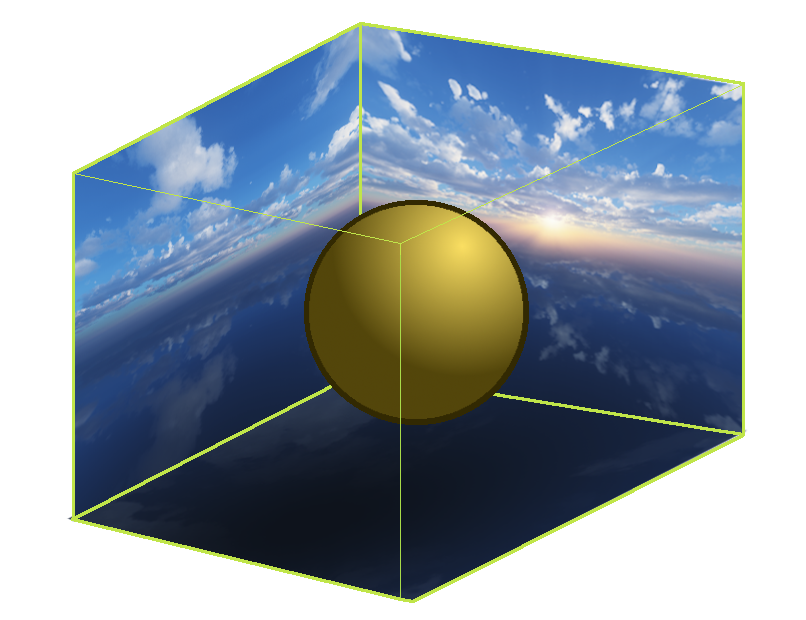
\includegraphics{edits/skybox}
            \captionof{figure}{The skybox cube as it is used in games.}
            \label{img:edits:skybox}
        \end{minipage}
    \hfill
        \begin{minipage}{0.45\linewidth}
            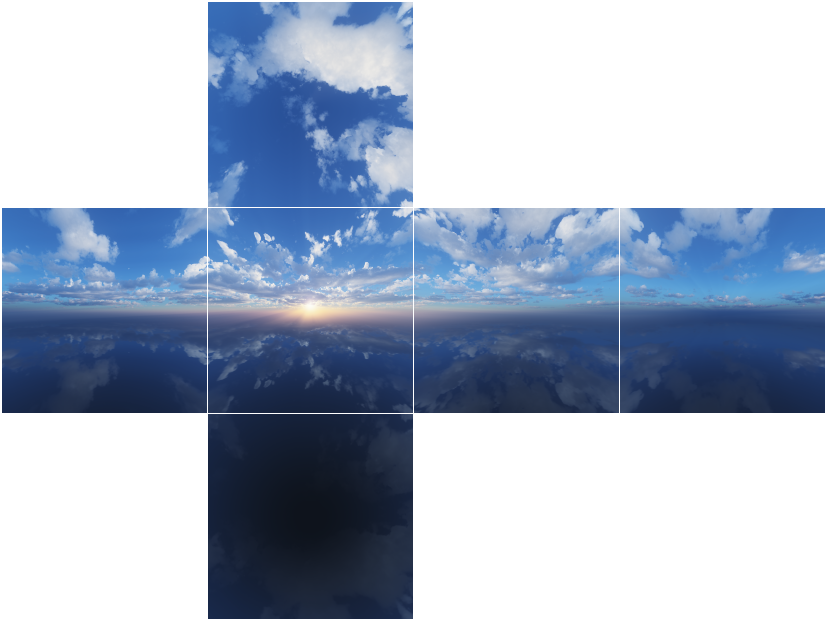
\includegraphics[width=\linewidth]{edits/skybox_layedout}
            \captionof{figure}{The polar sky dome images, folded out.}
            \label{img:edits:skybox_layedout}
        \end{minipage}
\end{figure}

\noindent
Besides rendering the sky, this of course allows clouds to be drawn right into the background. Also, in terms of performance, this is extremely cheap and efficient. On the other hand, it removes the ability for the clouds to move. 
They also have no volumetric body and no way of interaction with the game world whatsoever.
\\
This method does indeed give the scenery a more cloudy look, but what is missing is the "feel", or in other words the motion, interaction and lifelikeness of the clouds.

\subsubsection{Billboards}
Similar to the approach with the skybox, this technique also only uses 2D images of clouds. They are rendered individually and are always facing the camera. This is called \textit{\gls{billboard}ing}.
Now that each cloud is represented by its own game object, having a position in \gls{worldspace} as well as a scale and many other properties, it is possible to animate the clouds. For example, by moving the game objects in a circle around the world, the clouds seemingly "pass by".
\begin{figure}[H]
    \centering
        \begin{minipage}{0.48\linewidth}
            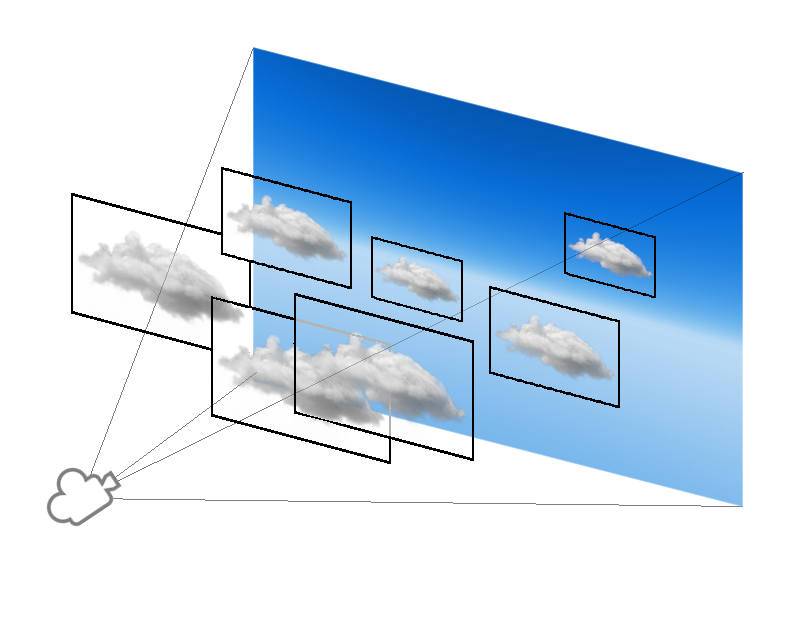
\includegraphics{edits/billboards}
            \captionof{figure}{A collection of 2D cloud billboards facing the camera.}
            \label{img:edits:billboards}
        \end{minipage}
    \hfill
        \begin{minipage}{0.45\linewidth}
            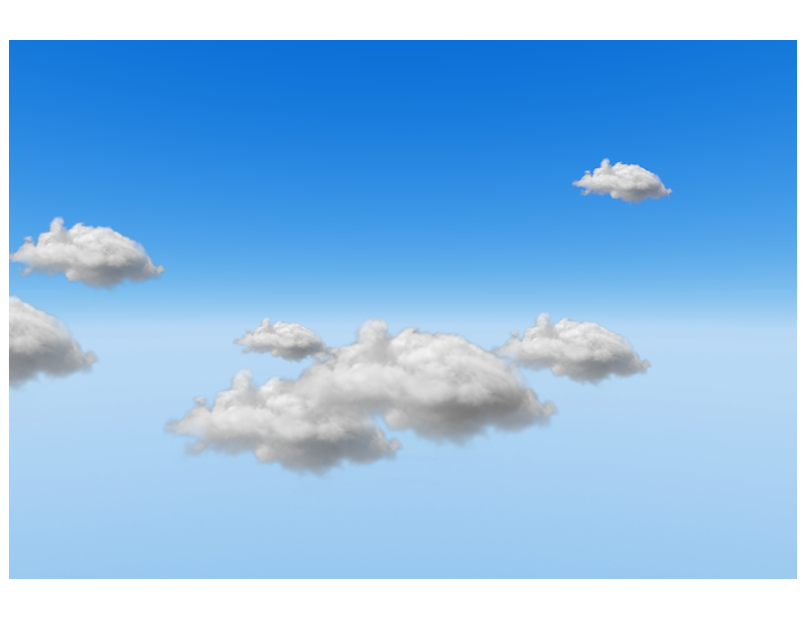
\includegraphics[width=\linewidth]{edits/billboards_rendered}
            \captionof{figure}{The rendered result of the image to the left.}
            \label{img:edits:billboards_rendered}
        \end{minipage}
\end{figure}
\noindent
Due to billboarding, the orientation is already given, making the overall time and effort of this technique quite advantageous to others.
\\
The major flaw of using billboards is of course that they are still 2D images, meaning they cannot really change appearance and therefore, do not evolve at all. 
Still, for many games, this technique suffices in the required diversity of background scenery and does not exceed the allowed performance share for such a task.

\subsubsection{Mesh-based Objects}
It is imaginable to simply use a \gls{polymesh} shaped like a cloud and render that like any other game object. By adding a texture, this would make for some decent looking clouds.
\\
However, the level of detail of such a polymesh is directly connected to the amount of vertices and faces that have to be processed every frame.
As seen in \autoref{img:rendered:cloud-mesh}, there are hundreds of polygons required to merely represent the basic shape of a realistic cloud.
If a similarly complex mesh is to be used for every cloud, a massive overhead is generated for objects that usually only contribute to the background of a game.
\begin{figure}[H]
    \centering
    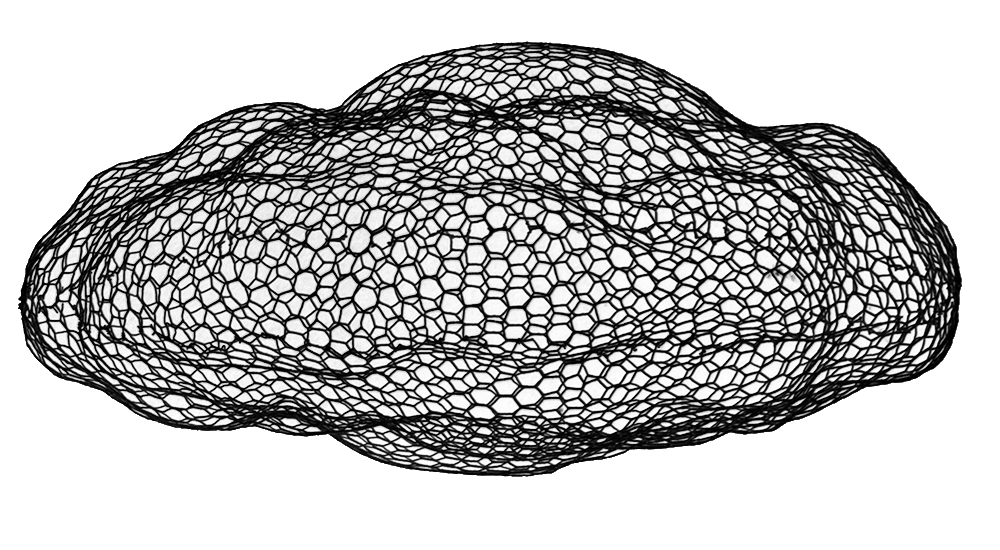
\includegraphics[width=0.5\linewidth]{rendered-cloud-mesh}
    \captionof{figure}{A \gls{polymesh} in the shape of an altocumulus cloud \cite{img:rendered:cloud-mesh}.}
    \label{img:rendered:cloud-mesh}
\end{figure}
\noindent
Apart from the performance impact, this method offers a volumetric, possibly interactable object just like any other 3D model does.
When massively decreasing the polygon count and therefore relinquishing the realistic look, mesh-based objects may be a viable solution for some \gls{lowpoly} games.
Otherwise, it is not reasonable to use this method.

\subsubsection{Volumetric Clouds}
Finally, clouds can be rendered via a technique called \textit{volumetric rendering}. The image below shows volumetric cloudscapes as seen in popular AAA titles.
The method itself is explained in detail in \sectionref{section:volumetric-rendering}.

\begin{figure}[H]
    \centering
    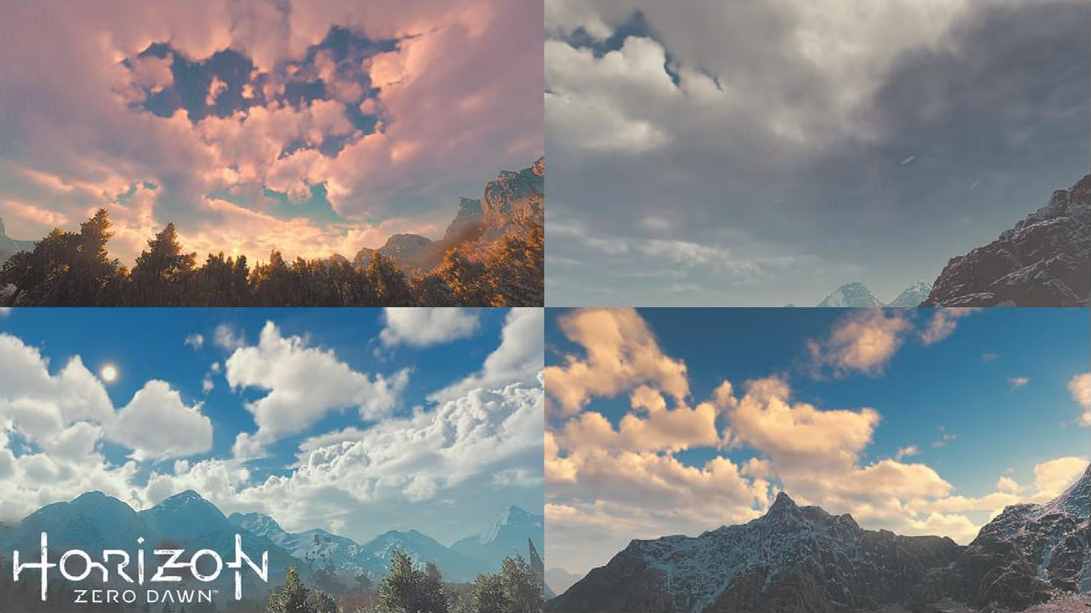
\includegraphics[width=\linewidth]{rendered-clouds-zerodawn}
    \captionof{figure}{Several volumetric cloudscapes from the game \textit{Horizon: Zero Dawn}, drawn in real time \protect\cite{img:rendered:clouds-zerodawn}.}
    \label{img:rendered:clouds-zerodawn}
\end{figure}
\clearpage

\section{Rendering techniques}

\subsection{Volumetric rendering}
\label{section:volumetric-rendering}

\subsubsection{Definition}
\Gls{volumetricrendering} describes a technique for generating a visual representation of data that is stored in a 3D volume. 
This especically comes to use for visual effects that are volumetric in nature, like fluids, clouds, fire, smoke, fog and dust, which all are extremely difficult or even impossible to model with geometric primitives.
\\
In addition to rendering such effects, volumetric rendering has become essential to scientific applications like medical imaging, for which a typical 3D data volume is a set of 2D slice images acquired by a CT (computed tomography) or MRI (magnetic resonance imaging) scanner.
\emptyline
The data volume is also called a \textit{\gls{scalarfield}} or \textit{\gls{vectorfield}}, which associates a scalar value, or \textit{\gls{voxel}}, to every point in the defined space.
This can be imagined like a 3D grid, where each point holds a single number. This number could, for example, represent the density of a cloud at that very point.
A \gls{voxel} may also consist of more than just a single value, but rather a set, like an RGB color.

\subsubsection{Ray Marching with constant step}
To actually render the volume data, a method called \textit{\gls{raymarching}} is used. With it, the surface distance of the volumetric data is approximated by creating a ray from the camera to the object for each fragment processed in the fragment shader. The ray is then extended into the volume of the object and stepped forward until the surface is reached.

\begin{figure}[H]
    \centering
    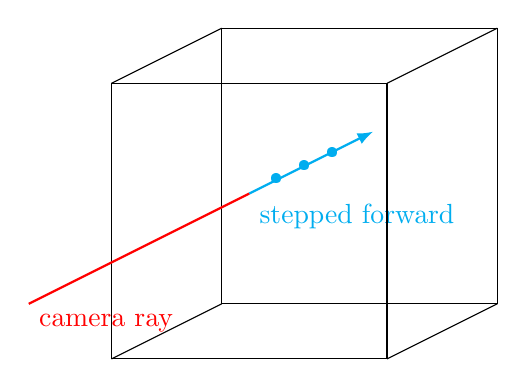
\begin{tikzpicture}[scale=0.7]
        \draw[-{Latex[length=2mm]},thick,cyan] (2.5,3) node[below right]{stepped forward} -- (4.75,4.125);
        \node[cyan] at (3.0,3.25) {\textbullet};
        \node[cyan] at (3.5,3.50) {\textbullet};
        \node[cyan] at (4.0,3.73) {\textbullet};
        
        \draw (0,0) -- (5,0) -- (5,5) -- (0, 5) -- (0, 0);
        \draw (2,1) -- (7,1) -- (7,6) -- (2, 6) -- (2, 1);
        \draw (0,0) -- (2,1); \draw (5,0) -- (7,1); \draw (5,5) -- (7,6); \draw (0,5) -- (2,6); 

        \draw[thick,red] (-1.5,1) node[below right]{camera ray} -- (2.5,3);

    \end{tikzpicture}
    \caption{A ray is created from the camera to the object. From there, it is extended into the volume.}
\end{figure}

\pagebreak
\noindent
In \gls{raymarching}, the algorithm only knows when it has reached the surface, or to be precise when it is inside the actual object volume.
\\
With this information, it is only possible to extend the ray in steps of a predefined length until the inside of the object is reached.
With a constant step, the approximation of the surface distance is exactly as precise as the size of the constant step.
\\
Once the ray is inside the actual volume, the functions returns the distance for this ray.

\begin{figure}[H]
    \centering
    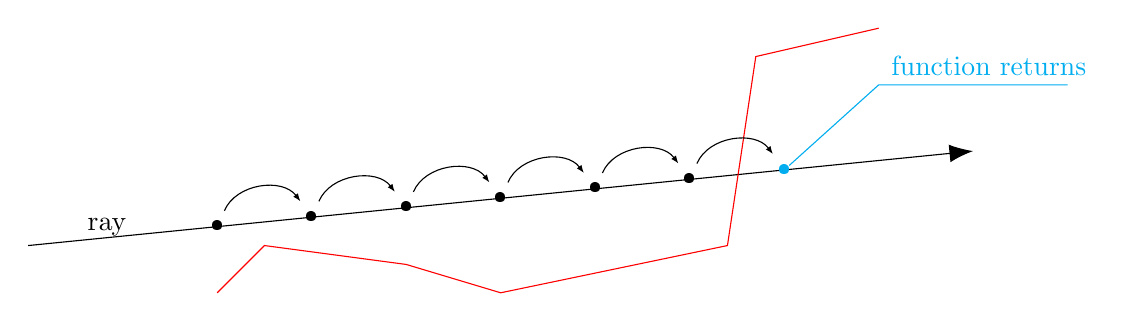
\begin{tikzpicture}[scale=1.2]
        \tikzset{edge/.style = {-{Latex[length=3mm]}}}
        \tikzset{smalledge/.style = {-{Latex[length=1mm]}}}

        % ray
        \draw[edge] (0,2) node[above,sloped,xshift=1cm]{ray} -- (10,3);
        \node (1) at (2,2.2) {\textbullet};
        \node (2) at (3,2.3) {\textbullet};
        \node (3) at (4,2.4) {\textbullet};
        \node (4) at (5,2.5) {\textbullet};
        \node (5) at (6,2.6) {\textbullet};
        \node (6) at (7,2.7) {\textbullet};
        \node[cyan] (7) at (8,2.8) {\textbullet};

        % surf dist
        \draw[red] (2,1.5) -- (2.5,2) -- (4,1.8) -- (5,1.5) -- (7.4,2) -- (7.7,4) -- (9,4.3);

        % ray steps
        \draw[smalledge] (1) edge[bend left=60] node [left]{} (2);
        \draw[smalledge] (2) edge[bend left=60] node [left]{} (3);
        \draw[smalledge] (3) edge[bend left=60] node [left]{} (4);
        \draw[smalledge] (4) edge[bend left=60] node [left]{} (5);
        \draw[smalledge] (5) edge[bend left=60] node [left]{} (6);
        \draw[smalledge] (6) edge[bend left=60] node [left]{} (7);

        % returns text
        \draw[cyan, shorten <=-0.2cm] (7) -- (9,3.7) -- (11,3.7) node[xshift=-1cm,above]{function returns};
        
        \end{tikzpicture}
    \caption{The function returns the evaluated surface distance, the precision of which being directly dependent on the step size.}
\end{figure}

\noindent
An implementation of this algorithm can be seen in \autoref{lst:shader:raymarch:spherehit}. Note that the volume to be rendered in this example is just a simple sphere.
So in order to check if the ray is inside the volume, the function \lstinline[language=HLSL]{sphereHit()} is used.
\begin{lstlisting}[language=HLSL, numbers=left, caption=The function returns true if the ray is inside the volume.,captionpos=b, label=lst:shader:raymarch:constantstep]
bool sphereHit(float3 position) {
    float4 sphere = float4(0, 1, 0, 1);
    return distance(sphere.xyz, position) < sphere.w;
}
\end{lstlisting}

\noindent
\newline 
With that given, the raymarch function is implemented like so:

\begin{lstlisting}[language=HLSL, numbers=left, caption=Ray march function with constant step.,captionpos=b, label=lst:shader:raymarch:spherehit]
fixed4 raymarch(float3 position, float3 direction)
{
    for (int i = 0; i < MAX_STEPS; i++)
    {
        if (sphereHit(position))
            return fixed4(1,0,0,1);
        
        position += normalize(direction) * STEP_SIZE;
    }
    
    return fixed4(0,0,0,1);
}
\end{lstlisting}


\subsubsection{Traditional Ray Marching}
It is obvious to see that, for a constant step ray march to result in an accurate approximation of the surface distance, the step size is required to be relatively small.
This has a direct impact on performance and thus, is not a viable solution for the problem.
\\
In traditional \gls{raymarching}, an optimization for that has been developed. The algorithm does not blindly step forward, but instead tries to get as close to the real distance as possible.
After the volume is reached, the step size is decreased and the ray steps out of the volume again. It then tries to approximate the surface distance by stepping back and forward repeatedly in continuously smaller steps, thus converging towards the exact intersection.
Once the step size falls below a certain threshold, the distance approximation is assumed to be precise enough and the value is returned for that ray march.

\begin{figure}[H]
    \centering
    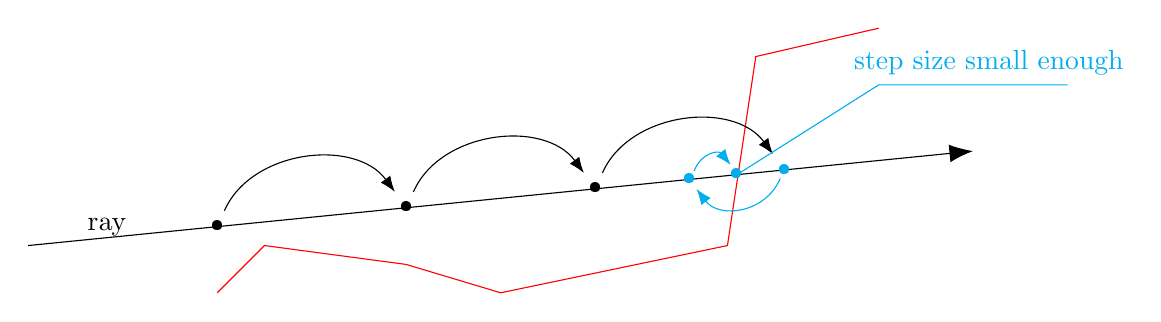
\begin{tikzpicture}[scale=1.2]
        \tikzset{edge/.style = {-{Latex[length=3mm]}}}
        \tikzset{smalledge/.style = {-{Latex[length=2mm]}}}

        % ray
        \draw[edge] (0,2) node[above,sloped,xshift=1cm]{ray} -- (10,3);
        \node (1) at (2,2.2) {\textbullet};
        \node (2) at (4,2.4) {\textbullet};
        \node (3) at (6,2.6) {\textbullet};
        \node[cyan] (4) at (8,2.8) {\textbullet};

        % surf dist
        \draw[red] (2,1.5) -- (2.5,2) -- (4,1.8) -- (5,1.5) -- (7.4,2) -- (7.7,4) -- (9,4.3);

        % reverse nodes
        \node[cyan] (5) at (7,2.7) {\textbullet};
        \node[cyan] (6) at (7.5,2.75) {\textbullet};

        % ray steps
        \draw[smalledge] (1) edge[bend left=60] node [left]{} (2);
        \draw[smalledge] (2) edge[bend left=60] node [left]{} (3);
        \draw[smalledge] (3) edge[bend left=60] node [left]{} (4);

        % rey reverse steps
        \draw[smalledge,cyan,shorten >=-0.1cm,shorten <=-0.1cm] (4) edge[bend left=60] node [left]{} (5);
        \draw[smalledge,cyan,shorten >=-0.1cm,shorten <=-0.1cm] (5) edge[bend left=60] node [left]{} (6);

        % close enough
        \draw[cyan, shorten <=-0.2cm] (6) -- (9,3.7) -- (11,3.7) node[xshift=-1cm,above]{step size small enough};
        
        \end{tikzpicture}
    \caption{The function returns the distance for this ray, which is the amount of steps times the step size.}
\end{figure}

\begin{lstlisting}[language=HLSL, numbers=left, caption=Traditional ray march function with converging surface distance approximation.,captionpos=b, label=lst:shader:raymarch:traditional]
fixed4 raymarch(float3 position, float3 direction)
{
    float stepSize = STEP_SIZE;
    float dirMultiplier = 1;
    for (int i = 0; i < MAX_STEPS; i++)
    {
        if (stepSize < MINIMUM_STEP_SIZE)
            return fixed4(1,0,0,1);

        if (sphereHit(position)) {
            // reduce step size by half and invert marching direction.
            stepSize /= 2;
            dirMultiplier = -1;
        } else {
            dirMultiplier = 1;
        }
        
        position += normalize(direction) * stepSize * dirMultiplier;
    }
    
    return fixed4(0,0,0,1);
}
\end{lstlisting}
\clearpage

\section{Common Algorithms}

\subsection{Noise Generation}
\label{section:noise-generation}
Nature's unpredictability and plays a big role in the diversity and appearance of cloudscapes. In shaders, an approach to that \textit{randomness} is used called \textit{\gls{noise}}.
In order to be able to implement random \gls{noise}, several important topics need to be looked into. It is best to start with randomness in computer science and how it is handled inside a shader program.

\subsubsection{Random Numbers}
As expected, there is no magic function which returns a pure random number inside the seemingly predictable and rigid code environment.
So the question how to generate randomness arises. 
\\
For this, the function $rnd(x) = fract(sin(x))$ is inspected, where $fract(x) = x - floor(x)$.

\begin{figure}[H]
    \centering
    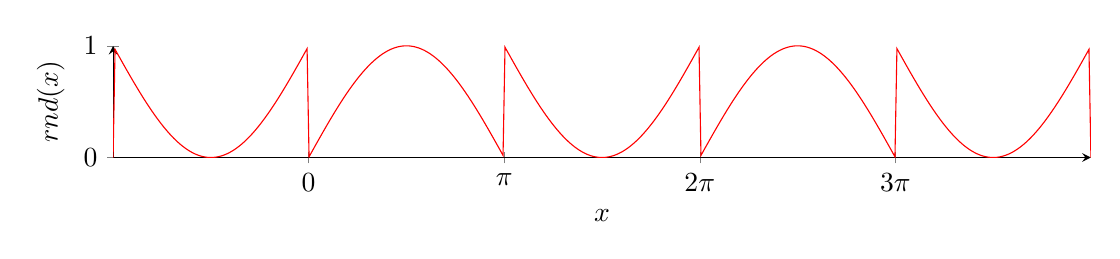
\begin{tikzpicture}[scale=1.0]
        \begin{axis}[
            samples=500,
            domain=-1*pi:4*pi,
            axis lines=left,
            xlabel=$x$,
            ylabel={$rnd(x)$},
            height=3cm,
            width=14cm,
            ytick={0,1},
            xtick={0,pi,2*pi,3*pi},
            xticklabels={$0$,$\pi$,$2\pi$,$3\pi$}
            ]
        \addplot[red] plot (\x, { sin(\x*1 r) - floor(sin(\x*1 r)) });
        \end{axis}
    \end{tikzpicture}
    \caption{Random numbers with the fractional value of sine of x.}
\end{figure}

\noindent
The sine values fluctuate between $-1$ and $1$, but with $fract$, only the fractional part is evaluated, turning the negative values in positive ones.
This effect can be used to get some pseudo-random values by "compressing" the function vertically or in other words, by increasing the frequency of the sine wave.
\\
The next figure displays the function $rnd(x) = fract(sin(x) * 10000)$.

\begin{figure}[H]
    \centering
    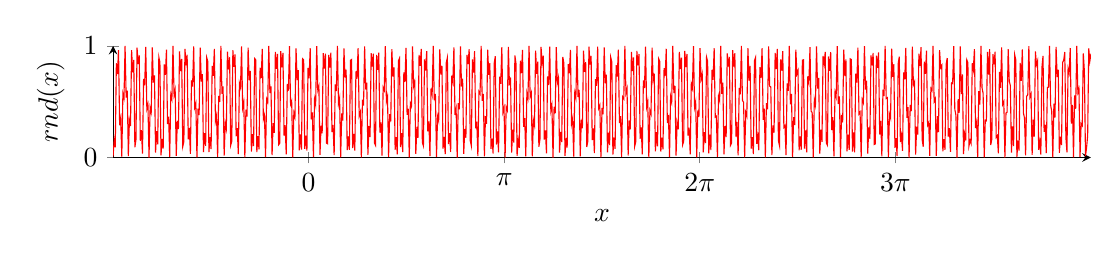
\begin{tikzpicture}[scale=1.0]
        \begin{axis}[
            samples=899,
            domain=-1*pi:4*pi,
            axis lines=left,
            xlabel=$x$,
            ylabel={$rnd(x)$},
            height=3cm,
            width=14cm,
            ytick={0,1},
            xtick={0,pi,2*pi,3*pi},
            xticklabels={$0$,$\pi$,$2\pi$,$3\pi$}
            ]
        \addplot[red] plot (\x, { sin(\x*10000 r) - floor(sin(\x*10000 r)) });
        \end{axis}
    \end{tikzpicture}
    \caption{Random numbers with the fractional value of sine of x multiplied by 10000.}
\end{figure}

\noindent
It is clearly visible that the function $rnd(x)$ became chaotic and seemingly random. However, it is noteworthy that $rnd(x)$ is still a deterministic function, which means for example $rnd(1.0)$ is always going to return the same value.
\clearpage

\printnoidxglossary 
\clearpage
\printbibliography[heading=bibintoc]
\clearpage
\phantomsection
\addcontentsline{toc}{section}{Listings}
\phantomsection
\addcontentsline{toc}{subsection}{Figures}
\listoffigures
\clearpage
\phantomsection
\addcontentsline{toc}{subsection}{Code Listings}
\lstlistoflistings

\end{document}
